\documentclass[11pt]{article}

\usepackage{verbatim}
\usepackage{amsmath}
\usepackage{amssymb}
\usepackage{setspace}
\usepackage[top=1in, bottom=1in, left=1.25in, right=1.25in]{geometry}
\usepackage{subfigure}
\usepackage{graphicx}
\usepackage{cite}
\usepackage[squaren]{SIunits}
\usepackage{listings}
\usepackage{csquotes}

\setlength{\parindent}{0pt} 	% remove the silly paragraph indents

% Sample figure
%\begin{figure}[h!]
%\centering
%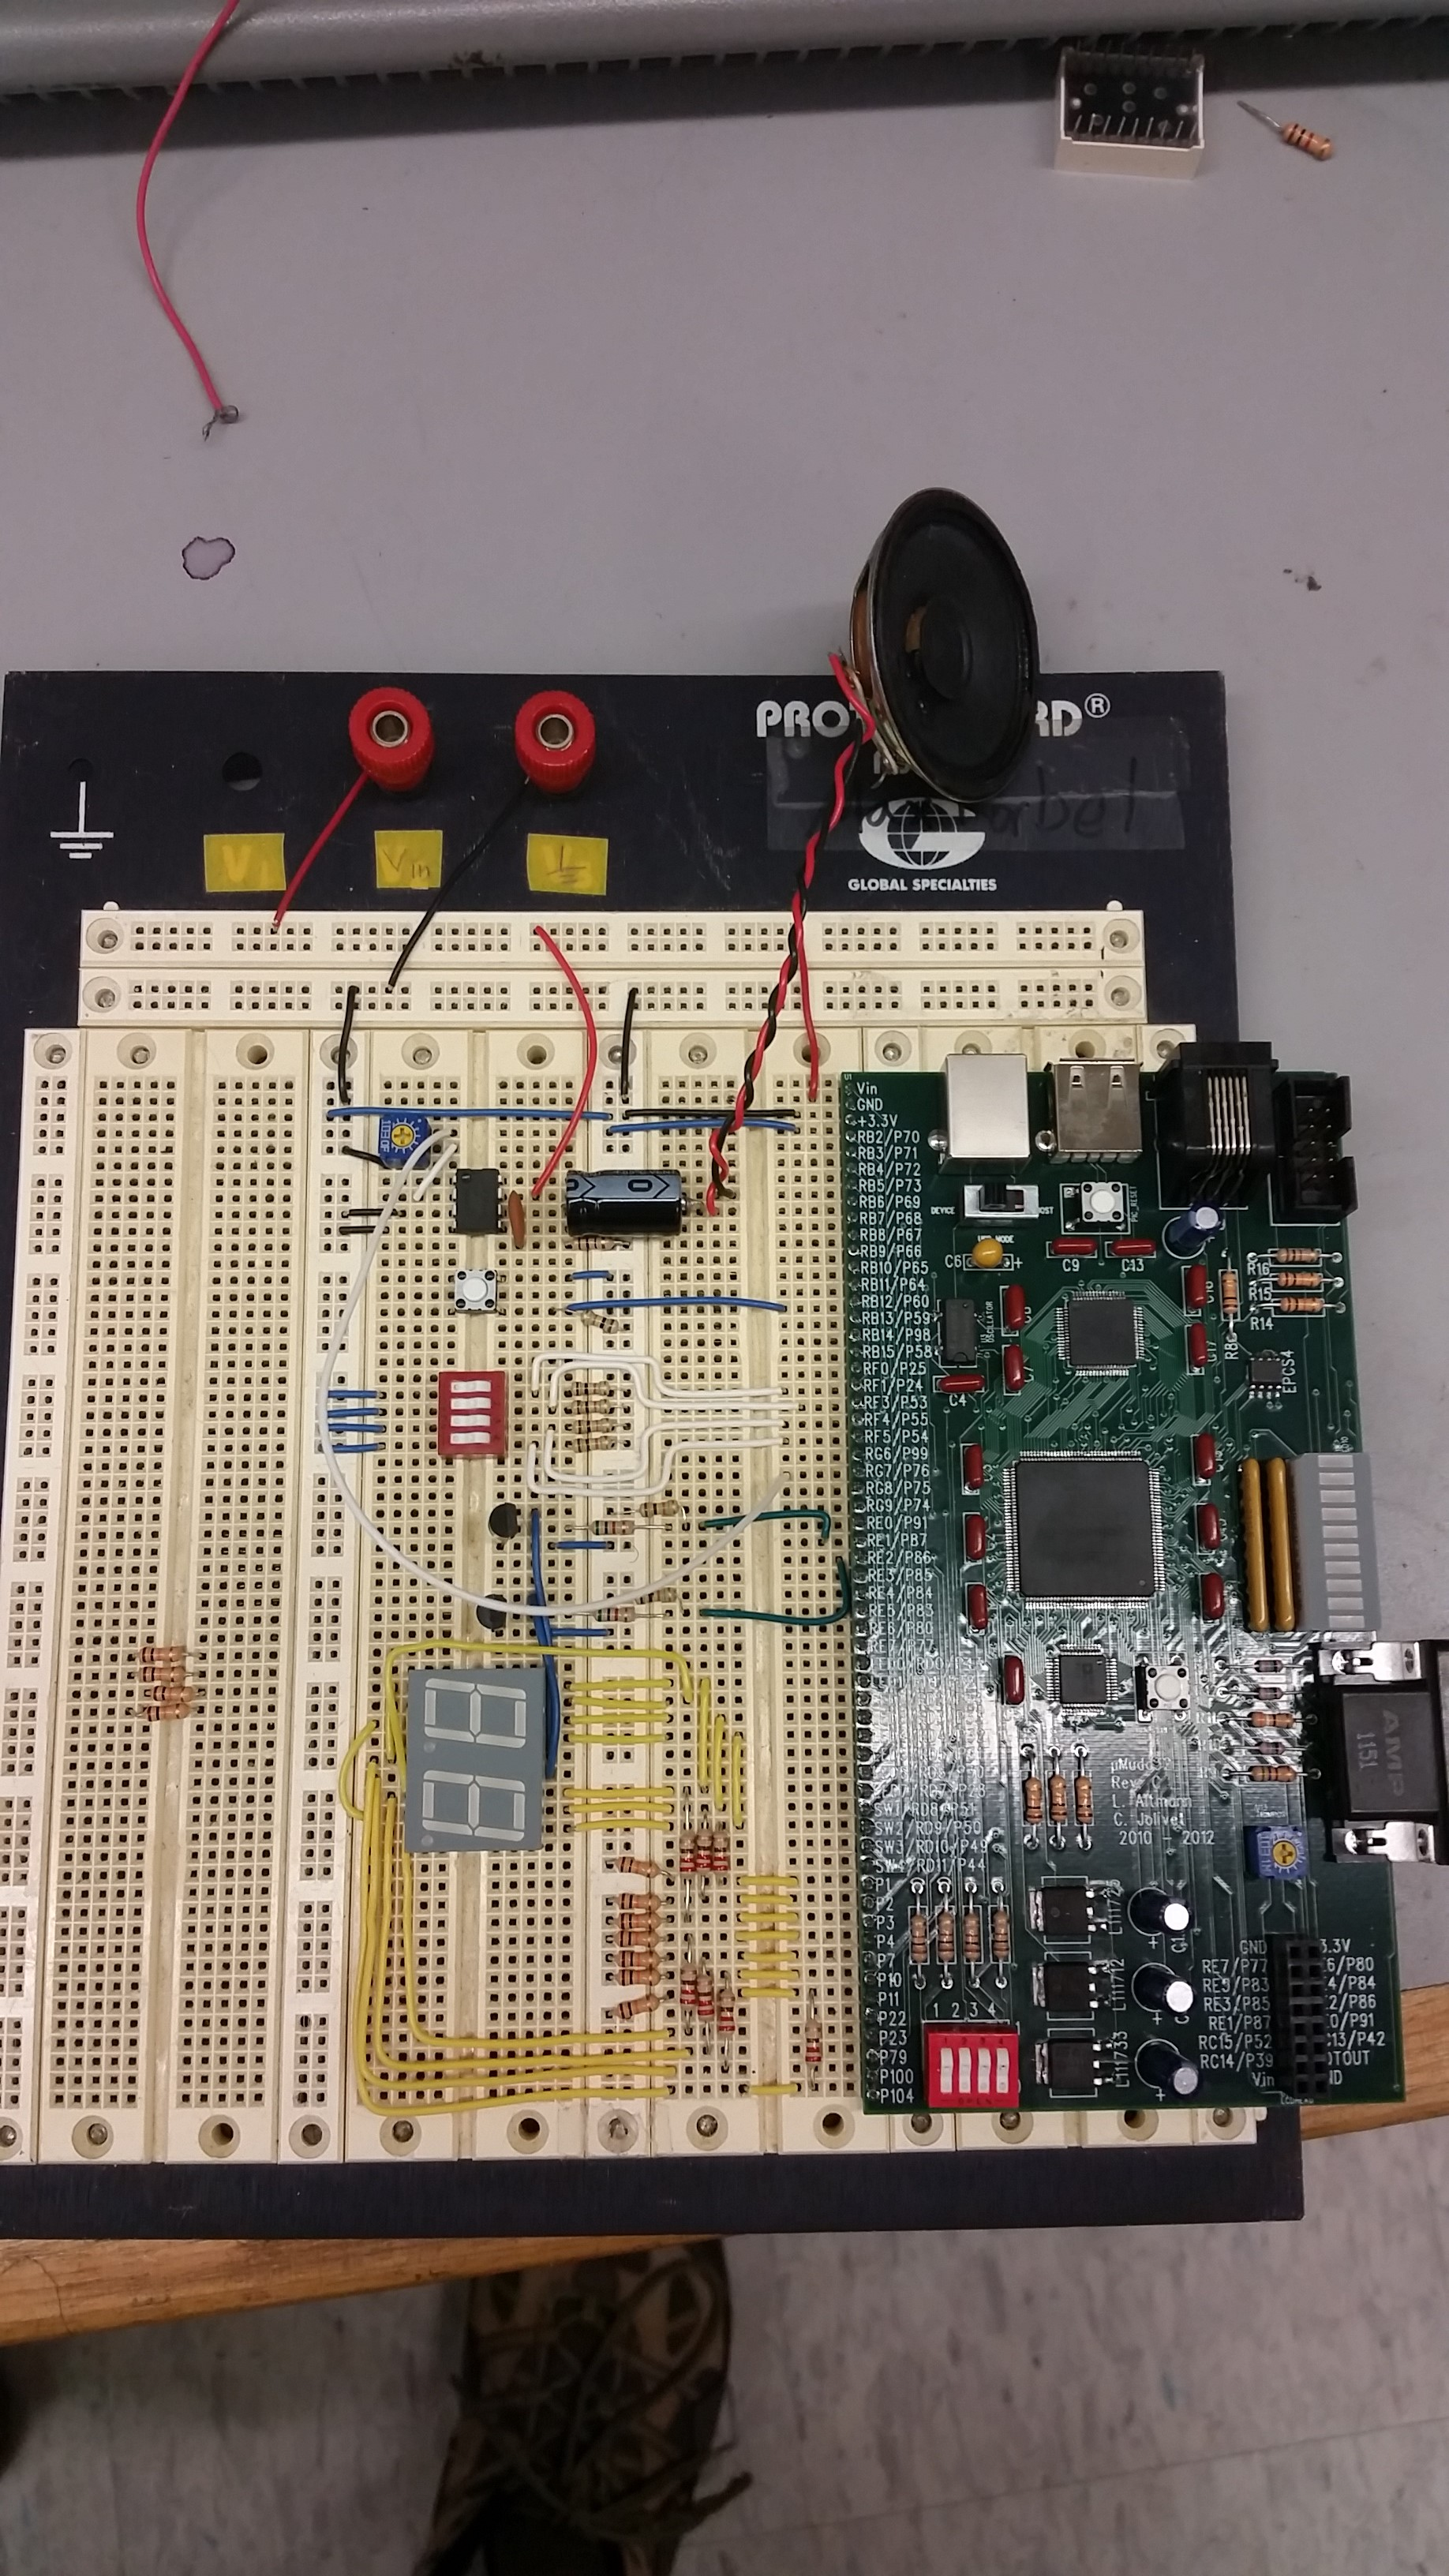
\includegraphics[scale=0.11]{board.jpg}
%\caption{The latest number entered on the keypad is displayed on the bottom display. The second latest number is displayed on the top.}
%\label{fig:board}
%\end{figure} 


\begin{document}



% ---------------------------------------
% Name section
% ---------------------------------------
\begin{flushleft}
Sherman Lam
\\E155
\\ \today
\end{flushleft}


% ---------------------------------------
% Title
% ---------------------------------------
\begin{center}
\begin{Large}
\textbf{Lab 4 Report: Microcontroller Sorting}
\end{Large}
\end{center}


% ---------------------------------------
% Start report
% ---------------------------------------


\section{Introduction}
\label{sec:intro}

In this lab, I used the PIC32 on the $\mu$Mudd32 to play a song that was loaded onto the PIC's flash memory. Two song segments were programmed into the PIC: Fur Elise and Reluctant Hero (from the anime, Attack on Titan). The PIC generated a square wave and drove the speaker through a LM380 audio amplifier.

\begin{figure}[h!]
\centering
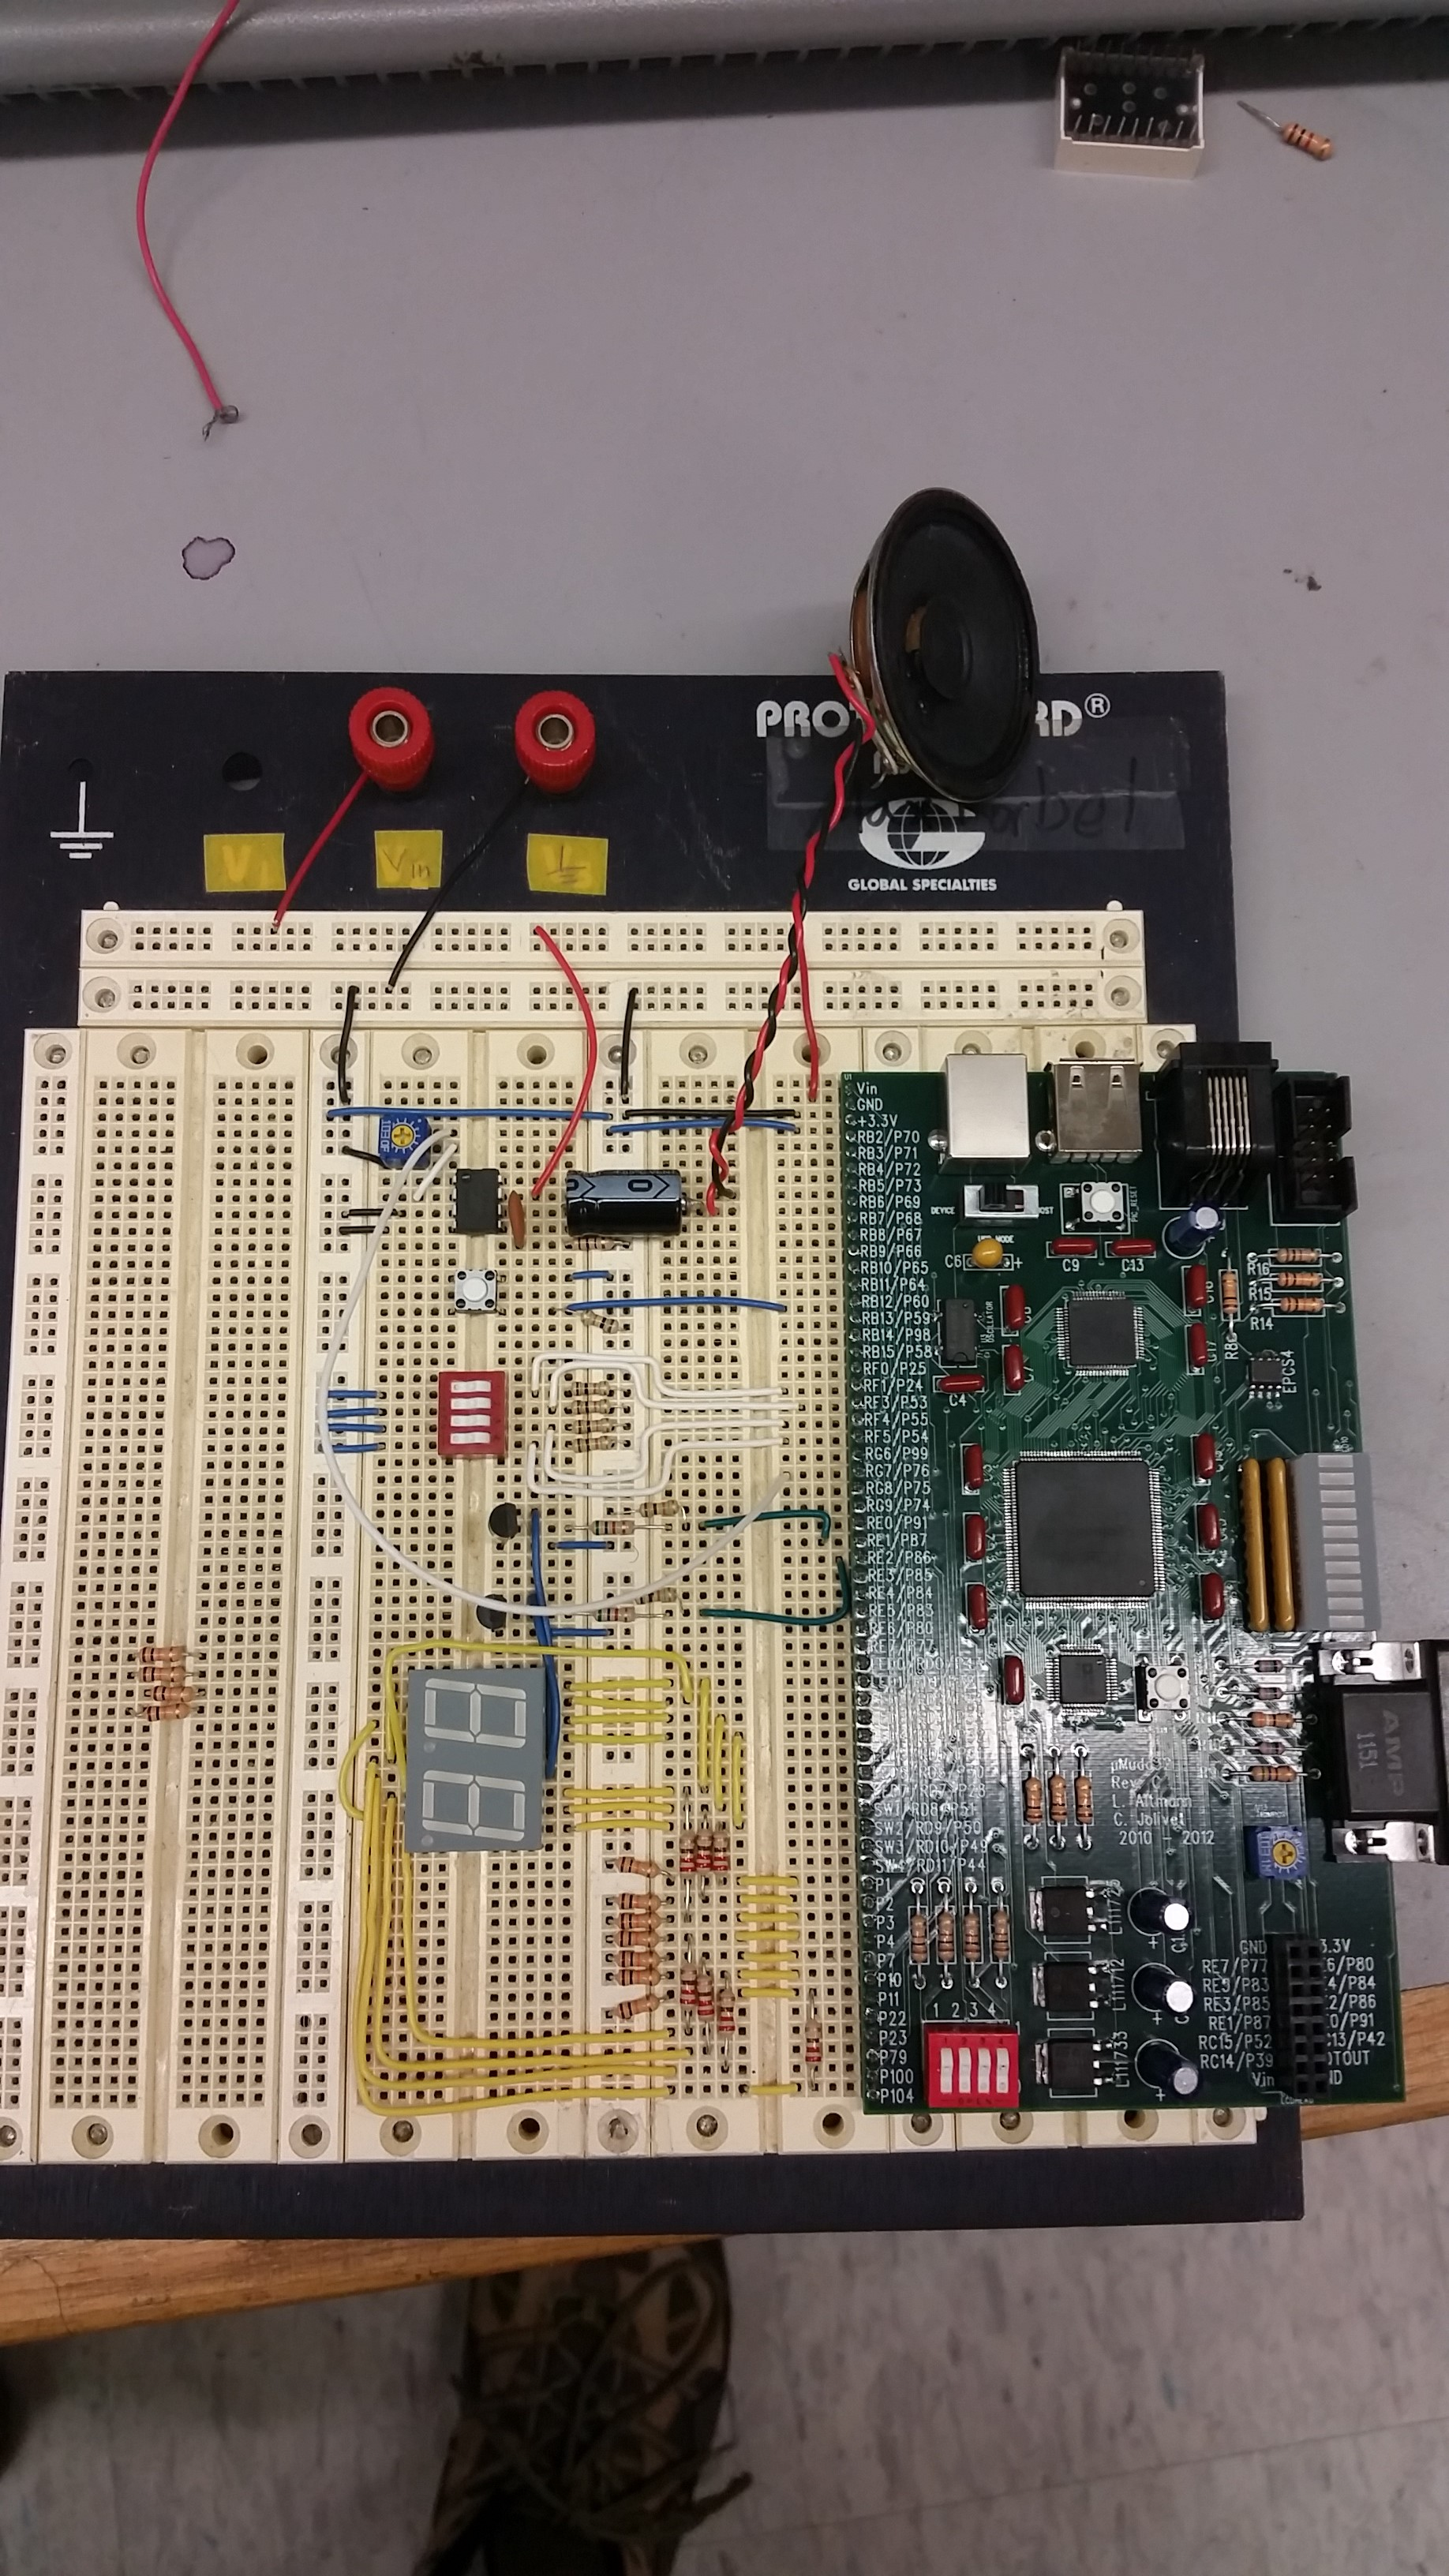
\includegraphics[scale=0.13]{board.jpg}
\caption{Complete development board with audio buffer / amplifier at the top of the breadboard.}
\label{fig:board}
\end{figure} 



\section{Design and Testing Methodology}

\subsection{Algorithm}

The music playing algorithm follows the following procedure outline:

\begin{enumerate}
	\item Setup timer 1
	\item Setup timer 2
	\item Load first period and duration from flash memory. Parse
	\item While the note duration has not been met, play the note
	\item Repeat from step 3 with new note.
\end{enumerate}

Here is some sudo-code that describes the method in slightly more detail.

\begin{lstlisting}[numbers=left,language=C,basicstyle=\footnotesize]
main(){
    // setup timers
    T1CON = 11xx_xxxx_xx11_xxx0;    // x = don't care
    T2CON = 11xx_xxxx_x010_xx0x;

    // setup outputs
    TRISG = 1111_1111_0111_1111;    // make port 7 an output

    // start playing the song
    int i = 0;
    while(true){
        int word = _notes[i];

        // check for end of song
        if (word == 0){
            break;
        }

        int halfPeriod = word[15:8];
        int duration = word[7:0];

        // play for duration
        TMR1 = 0
        TMR2 = 0
        while(TMR1 < duration){
            //toggle according to the period
            if (TMR2 >= halfPeriod){
                //toggle output
                PORTG[7] = ~PORTG[7];
                TMR2 = 0;
            }
        }
        //move to next note
        i++;
    }
}

\end{lstlisting}


\subsection{Timing}

The clock on the $\mu$Mudd32 operates at 40Hz. The prescalar for the PIC's peripheral clock was set to 1:8. This means that the peripheral clock will run at $\frac{40MHz}{8} = 5MHz$. \\

Timer 1's prescalar is set to 1:256. This makes this timer run at $\frac{5MHz}{256} = 19.5kHz$ or a period of 5.12$\mu s$. This timer is used to keep track of the duration of each note. Let each count of timer 1 be $\tau_{0}$. The duration, $\tau_{0}$, of each type of note is given in Figure \ref{fig:freq_and_dur}. \\

Timer 2's prescalar is set to 1:4. This allows the timer to run at $\frac{5MHz}{4} = 1.25MHz$ or a period of 0.8$\mu s$. Timer 2 is used to keep track of the period of each note. Let each count of timer 1 be $\tau_{1}$. The period, in units of $\tau_{1}$, are given in Figure \ref{fig:freq_and_dur}. Let's use A4 to check the timing. This has a frequency of $440Hz$ and period of 0x58C$\tau_{1}$. Converting the period to seconds yields $1420(0.8\mu s) = 1.136ms$. This corresponds to a frequency of $880Hz$. Note that this is double the real frequency of the note. Also note that to generate a square wave with frequency $F$, the pin needs to be toggled at a frequency of $2F$. Thus, Figure \ref{fig:freq_and_dur} lists the toggling period of the pin. \\

\begin{figure}[h!]
\centering
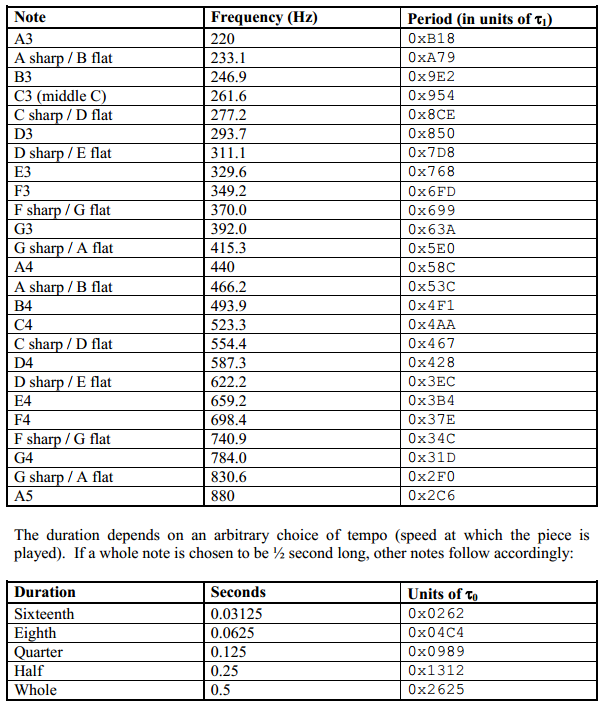
\includegraphics[scale=0.8]{notes_and_duration.png}
\caption{Mapping from note frequency and duration to periods of timers 1 and 2.}
\label{fig:freq_and_dur}
\end{figure} 



\subsection{Using a Speaker}

The output pins of the PIC32 can only output 25mA (from PIC32 datasheet). However, the speaker draws much more. A 2W speaker operating at 5V would need to draw $\frac{2W}{5V} = 400mA$. This would surely burn out an I/O pin on the PIC32. So, I used an audio amplifier to drive the speaker. The lab recommends using the LM386. From the LM386 datasheet, I found a recommended circuit (see Figure \ref{fig:amp_sch}). \\

\begin{figure}[h!]
\centering
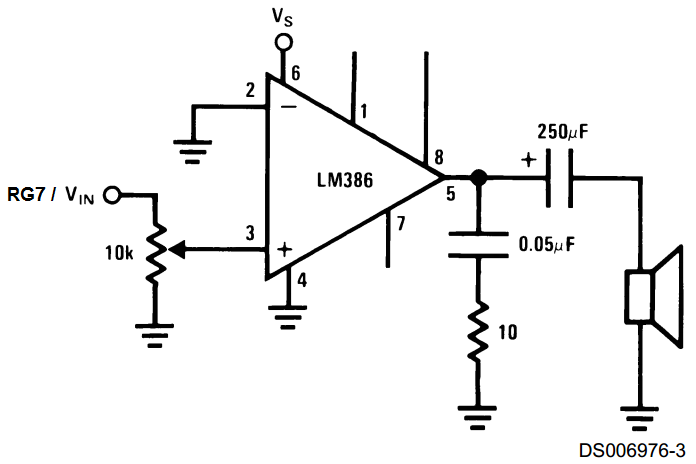
\includegraphics[scale=0.7]{amp.png}
\caption{Basic amplifier configuration.}
\label{fig:amp_sch}
\end{figure} 
 
However, the lab was out of LM386 ICs so I used an LM380 amplifier. The LM380 is similar in function to the LM386 but has different pin layouts. Using the pinout for the LM380 from Figure \ref{fig:LM380_pin}, I replicated the circuit presented in Figure \ref{fig:amp_sch}. \\
 
\begin{figure}[h!]
\centering
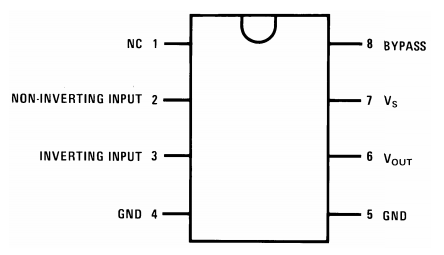
\includegraphics[scale=0.8]{LM380_pin.png}
\caption{Basic amplifier configuration.}
\label{fig:LM380_pin}
\end{figure} 


\clearpage


\section{Technical Documentation}

\subsection{MIPS Code - Playing a Song from Flash Memory}

\begin{lstlisting}[numbers=left,basicstyle=\footnotesize]
/* This code plays music!

Author: Sherman Lam
Email: slam@g.hmc.edu
Date: 10-9-2014
*/


# REGISTER USE
# t0 = register address
# t1 = register value
# t2 = masking operations
# t3 = note period
# t4 = duration
# t5 = address of note
# t6 = algebra intermediate values
# s0 = PORTB address
# s1 = PORTB output



# load a header file for pin / register definitions
#include <P32xxxx.h>

# Define constants
#define PBDIV 0x3       # prescaler for peripheral clock. 0x3 = 1:8

# Define main function
.global main

# Compiler instructions
.text # store the code in the main program section of RAM
.set noreorder # do not let the compiler reorganize your code

# Main program
.ent main # Start function block
main:
    nop

    # setup peripheral clock. Default is 1:8 but let's set it anyways
    # OSCCON:
    #   bit 20-19 = 11 -> 1:8 prescalar
    #la      t0, OSCCON      # OSCCON = oscillator control register
    #lw      t1, 0(t0)       # get the value of OSCCON
    #li      t2, 0xFFE7FFFF  # mask for clearing PBDIV, which is bits 20-19
    #and     t1, t1, t2      # use the mask to set PBDIV to 00
    #li      t2, 0x3         # load mask for setting PBDIV
    #sll     t2, t2, 19      # shift the mask to the right location
    #or      t1, t1, t2      # set desired PBDIV
    #sw      t1, 0(t0)       # load new value into OSCCON
    # THIS DOESN"T WORK. GETS OVERRIDED BY CONFIG BITS

    # setup timer 1 (for 1 unit of signal duration = 51.2us)
    # T1CON:
    #   bit 15  = 1     -> on
    #       14  = 1     -> freeze on debug exception
    #       5-4 = 11    -> 1:256 prescaler
    #       1   = 0     -> use peripheral clock
    la      t0, T1CON       # load address of T1CON
    lw      t1, 0(t0)       # get the value of T1CON
    andi    t1, t1, 0xFFFD  # use a mask to set the 0 bit
    ori     t1, t1, 0xC030  # use a mask to set the 1 bits
    sw      t1, 0(t0)       # load new value to T1CON

    # setup timer 2 (for half signal period = 0.8us)
    # T2CON:
    #   bit 15  = 1     -> on
    #       14  = 1     -> freeze on debug exception
    #       6-4 = 010   -> 1:256 prescaler
    #       1   = 0     -> use peripheral clock
    la      t0, T2CON       # load address of T2CON
    lw      t1, 0(t0)       # get the value of T2CON
    andi    t1, t1, 0xFFAD  # use a mask to set the 0 bits
    ori     t1, t1, 0xC020  # use a mask to set the 1 bits
    sw      t1, 0(t0)       # load new value to T2CON

    # init some variables
    la      t5, _notes      # starting address of _notes

    # init output
    la      t0, TRISG       # load address of TRISG
    lw      t1, 0(t0)       # get value of TRISB
    andi    t1, t1, 0xFF00  # set RG7 as output
    sw      t1, 0(t0)       # store to TRISB
    la      s0, PORTG       # load address of PORTB
    sw      zero, 0(s0)     # start at 0

    # start main loop for playing song
    play:
        nop
        # read the note and duration. If there is no note, end
        lw      t6, 0(t5)             # load notes and duration into algebra register
        beq     t6, zero, end         # branch if there are no more notes
        li      t2, 0xFFFF0000        # mask for duration
        and     t4, t6, t2            # mask off to get duration
        srl     t4, t4, 16            # shift to lower 16bits to get duration
        andi    t3, t6, 0xFFFF        # mask off the note
        li      t6, 0x2               # load 2 into t6
        mul     t4, t4, t6            # multiply duration by 2

        # reset timer 1
        la      t0, TMR1          # get address of timer 1
        sw      zero, 0(t0)       # reset timer to 0

        # reset timer 2
        la      t0, TMR2        # get address of timer 2
        sw      zero, 0(t0)       # reset timer to 0

        # poll the timer until the duration has been met
        dur:
            la      t0, TMR1        # get address of timer 1
            lw      t1, 0(t0)       # poll timer 1
            beq     t1, t4, next    # check if timer 1 has reached duration
            nop

            # while the duration is being held, keep playing the notes
            note:
                la      t0, TMR2        # get address of timer 2
                lw      t1, 0(t0)       # poll timer 2
                slt     t6, t1, t3      # check if time is less than the period
                bne     t6, zero, dur   # if not time to toggle speaker, check duration
                nop
                # toggle!
                li      t6, 0xFFFF      # load -1 into t6
                xor     s1, s1, t6      # xor with -1. This inverts all the bits
                andi    s1, s1, 0x0080  # use mask to only get RG7
                la      s0, PORTG       # load address of PORTG
                sw      s1, 0(s0)       # write the value to PORTG.
                la      t0, TMR2        # get address of timer 2
                sw      zero, 0(t0)     # reset timer 2
                j       dur             # check duration
                nop

        # figure out next offset
        next:
            la      t0, TMR1            # get address of timer 1
            sw      zero, 0(t0)         # reset timer 1
            addi    t5, t5, 4           # get next note's address
            j       play                # play the next note
            nop

    end:
        nop
        jr      ra                  # jump to return address.


# end the function
.end main
\end{lstlisting}

\subsubsection{Loading Fur Elise to Flash}

\begin{lstlisting}[numbers=left,basicstyle=\footnotesize]
# Song notes
    .section .rodata  # Store this information in FLASH instead of RAM
_notes:
    .HWORD 0x3b4, 0x989 # Data
    .HWORD  0x3ec, 0x989
    .HWORD 0x3b4, 0x989
    .HWORD 0x3ec, 0x989
    .HWORD 0x3b4, 0x989
    .HWORD 0x4f1, 0x989
    .HWORD 0x428, 0x989
    .HWORD 0x4aa, 0x989
    .HWORD 0x58c, 0x1312
    .HWORD 0x000, 0x989
    .HWORD 0x954, 0x989
    .HWORD 0x768, 0x989
    .HWORD 0x58c, 0x989
    .HWORD 0x4f1, 0x1312
    .HWORD 0x000, 0x989
    .HWORD 0x768, 0x989
    .HWORD 0x5e0, 0x989
    .HWORD 0x4f1, 0x989
    .HWORD 0x4aa, 0x1312
    .HWORD 0x000, 0x989
    .HWORD 0x768, 0x989
    .HWORD 0x3b4, 0x989
    .HWORD 0x3ec, 0x989
    .HWORD 0x3b4, 0x989
    .HWORD 0x3ec, 0x989
    .HWORD 0x3b4, 0x989
    .HWORD 0x4f1, 0x989
    .HWORD 0x428, 0x989
    .HWORD 0x4aa, 0x989
    .HWORD 0x58c, 0x1312
    .HWORD 0x000, 0x989
    .HWORD 0x954, 0x989
    .HWORD 0x768, 0x989
    .HWORD 0x58c, 0x989
    .HWORD 0x4f1, 0x1312
    .HWORD 0x000, 0x989
    .HWORD 0x768, 0x989
    .HWORD 0x4aa, 0x989
    .HWORD 0x4f1, 0x989
    .HWORD 0x58c, 0x1312
    .HWORD 0x000, 0x989
    .HWORD 0x4f1, 0x989
    .HWORD 0x4aa, 0x989
    .HWORD 0x428, 0x989
    .HWORD 0x3b4, 0x1c9c
    .HWORD 0x63a, 0x989
    .HWORD 0x37e, 0x989
    .HWORD 0x3b4, 0x989
    .HWORD 0x428, 0x1c9c
    .HWORD 0x6fd, 0x989
    .HWORD 0x3b4, 0x989
    .HWORD 0x428, 0x989
    .HWORD 0x4aa, 0x1c9c
    .HWORD 0x768, 0x989
    .HWORD 0x428, 0x989
    .HWORD 0x4aa, 0x989
    .HWORD 0x4f1, 0x1312
    .HWORD 0x000, 0x989
    .HWORD 0x768, 0x989
    .HWORD 0x3b4, 0x989
    .HWORD 0x000, 0x989
    .HWORD 0x000, 0x989
    .HWORD 0x3b4, 0x989
    .HWORD 0x1da, 0x989
    .HWORD 0x000, 0x989
    .HWORD 0x000, 0x989
    .HWORD 0x3ec, 0x989
    .HWORD 0x3b4, 0x989
    .HWORD 0x000, 0x989
    .HWORD 0x000, 0x989
    .HWORD 0x3ec, 0x989
    .HWORD 0x3b4, 0x989
    .HWORD 0x3ec, 0x989
    .HWORD 0x3b4, 0x989
    .HWORD 0x3ec, 0x989
    .HWORD 0x3b4, 0x989
    .HWORD 0x4f1, 0x989
    .HWORD 0x428, 0x989
    .HWORD 0x4aa, 0x989
    .HWORD 0x58c, 0x1312
    .HWORD 0x000, 0x989
    .HWORD 0x954, 0x989
    .HWORD 0x768, 0x989
    .HWORD 0x58c, 0x989
    .HWORD 0x4f1, 0x1312
    .HWORD 0x000, 0x989
    .HWORD 0x768, 0x989
    .HWORD 0x5e0, 0x989
    .HWORD 0x4f1, 0x989
    .HWORD 0x4aa, 0x1312
    .HWORD 0x000, 0x989
    .HWORD 0x768, 0x989
    .HWORD 0x3b4, 0x989
    .HWORD 0x3ec, 0x989
    .HWORD 0x3b4, 0x989
    .HWORD 0x3ec, 0x989
    .HWORD 0x3b4, 0x989
    .HWORD 0x4f1, 0x989
    .HWORD 0x428, 0x989
    .HWORD 0x4aa, 0x989
    .HWORD 0x58c, 0x1312
    .HWORD 0x000, 0x989
    .HWORD 0x954, 0x989
    .HWORD 0x768, 0x989
    .HWORD 0x58c, 0x989
    .HWORD 0x4f1, 0x1312
    .HWORD 0x000, 0x989
    .HWORD 0x768, 0x989
    .HWORD 0x4aa, 0x989
    .HWORD 0x4f1, 0x989
    .HWORD 0x58c, 0x2625
    .HWORD 0x000, 0x000
\end{lstlisting}

\subsubsection{Loading Reluctant Heros (from Attack on Titan anime) to Flash Memory}
\begin{lstlisting}[numbers=left,basicstyle=\footnotesize]
# Song notes
    .section .rodata  # Store this information in FLASH instead of RAM
_notes:
    .HWORD 0x428, 0x989     # D4
    .HWORD 0x467, 0x989     # C4#
    .HWORD 0x428, 0x989     # D4
    .HWORD 0x3b4, 0x989     # E4

    .HWORD 0x34c, 0x1312    # F4#
    .HWORD 0x4f1, 0x989     # B4
    .HWORD 0x428, 0x1312    # D4
    .HWORD 0x4f1, 0x989     # B4
    .HWORD 0x428, 0x989     # D4
    .HWORD 0x3b4, 0x989     # E4
    
    .HWORD 0x34c, 0x1312    # F4#
    .HWORD 0x4f1, 0x989     # B4
    .HWORD 0x428, 0x1312    # D4
    .HWORD 0x428, 0x989     # D4
    .HWORD 0x428, 0x989     # D4
    .HWORD 0x2c6, 0x1312    # A5

    .HWORD 0x31d, 0x1312    # G4
    .HWORD 0x31d, 0x1312    # G4
    .HWORD 0x34c, 0x1312    # F4#
    .HWORD 0x34c, 0x1312    # F4#

    .HWORD 0x3b4, 0x1312    # E4
    .HWORD 0x428, 0x1312    # D4
    .HWORD 0x4f1, 0x989     # B4
    .HWORD 0x428, 0x989     # D4
    .HWORD 0x3b4, 0x989     # E4

    .HWORD 0x34c, 0x1312    # F4#
    .HWORD 0x4f1, 0x989     # B4
    .HWORD 0x428, 0x1312    # D4
    .HWORD 0x4f1, 0x989     # B4
    .HWORD 0x428, 0x989    # D4
    .HWORD 0x3b4, 0x989     # E4

    .HWORD 0x34c, 0x1312    # F4#
    .HWORD 0x4f1, 0x989     # B4
    .HWORD 0x428, 0x1312    # D4
    .HWORD 0x428, 0x989    # D4
    .HWORD 0x467, 0x989     # C4#
    .HWORD 0x428, 0x1312    # D4

    .HWORD 0x3b4, 0x1312     # E4
    .HWORD 0x428, 0x1312    # D4
    .HWORD 0x428, 0x989    # D4
    .HWORD 0x467, 0x989     # C4#
    .HWORD 0x428, 0x1312    # D4

    .HWORD 0x34c, 0x1312    # F4#
    .HWORD 0x3b4, 0x1312     # E4
    

    .HWORD 0x0, 0x0         # stop
\end{lstlisting}

\clearpage

\subsection{Timer 1 and Timer 2 Registers}

\begin{figure}[h!]
\centering
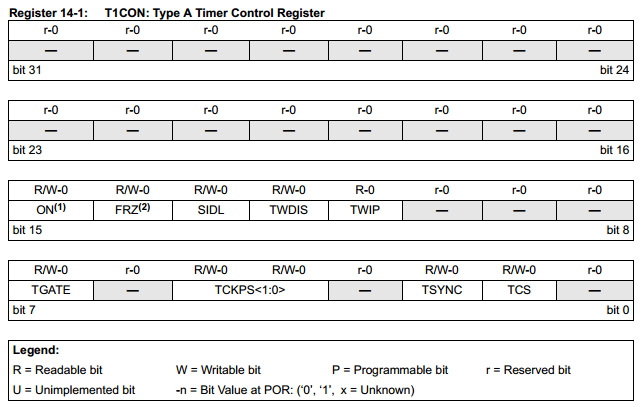
\includegraphics[scale=0.8]{T1CON.png}
\caption{Control Register for T1CON.}
\label{fig:t1con}
\end{figure} 

\begin{figure}[h!]
\centering
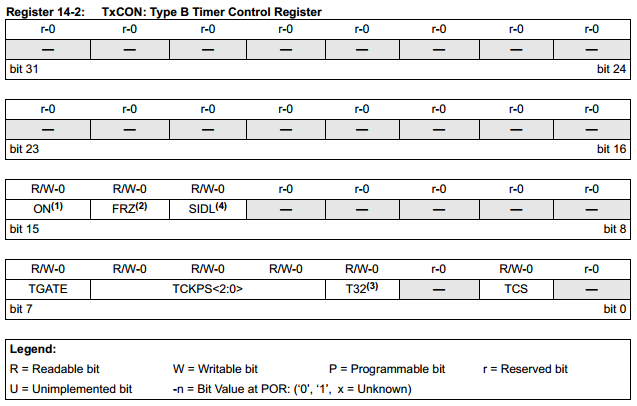
\includegraphics[scale=0.8]{T2CON.png}
\caption{Control Register for T2CON.}
\label{fig:t2con}
\end{figure} 


\clearpage

\section{Results and Discussion}

Music playing works! Since the tempo was arbitrary chosen when \ref{fig:freq_and_dur} was created, Fur Elise was too fast. So, I doubled the periods to slow down the song to an appropriate pace. \\

I also converted the first several measures of "Reluctant Hero" into units of $\tau_{0}$ and $\tau_{1}$. This also plays as expected.


\section{Conclusion}

\subsection{Time Spent}

\begin{description}
	\item[Programming, Simulating] 6 hrs
 	\item[Writing Report] 3hrs
	\item[Total Time Spent] 9hrs
\end{description}

\subsection{Suggestions for lab}

No suggestions for the lab.

\end{document}

